\chapter{Grundlagen}
\label{grundlagen}

\textit{Ein Verständnis der Möglichkeiten ist der Schlüssel […] zur Gestaltung und Durchführung von Text-Analysen} \cite[S. vii]{Anandarajan}.
%\epigraph{Ein Verständnis der Möglichkeiten ist der Schlüssel […] zur Gestaltung und Durchführung von Text-Analysen.}{--- \textup{aus} \cite[S. vii]{Anandarajan}}

\section{Künstliche Intelligenz, Machine Learning \& Deep Learning}

Abbildung \ref{Abbildung:kelleher} gibt einen groben Überblick darüber, wie die in dieser Überschrift genannten Begriffe zu verstehen sind und in welcher Beziehung sie zueinander stehen. 

\begin{figure}[h]
\centering
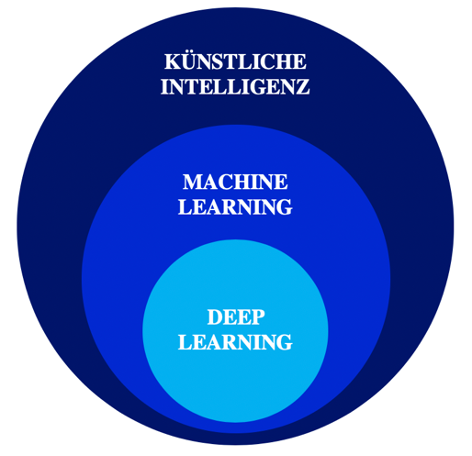
\includegraphics[scale=1.0]{content/pics/Picture_2.png}
\caption{Zusammenhang von KI, ML und Deep Learning. Eigene Erstellung in Anlehnung an \cite{Kelleher}}
\label{Abbildung:kelleher}
\end{figure}

Das Ziel der künstlichen Intelligenz ist es Systeme aufzubauen, die Aufgaben lösen können, die Intelligenz auf Niveau des Menschen voraussetzen. Machine Learning wird dabei als Teilmenge bzw. Teildisziplin der künstlichen Intelligenz eingeordnet \cite[S. 14]{Gupta}.

Machine Learning ermöglicht es Computern, aus Erfahrungen beziehungsweise aus Aufzeichnungen Regeln zu lernen, ohne explizit programmiert zu werden \cite{samuel}. Gängig ist im Bereich Machine Learning eine Unterscheidung zwischen drei Arten des Lernens: dem überwachten Lernen, dem unüberwachten Lernen, und dem sogenannten Reinforcement Learning. 

Beim überwachten Lernen existiert in Trainingsdaten für jedes Beispiel eine Beschriftung. Mit Hilfe der Beschriftungen (oder auch Klassen) kann nun beispielsweise ein Klassifikationsmodell gelernt werden. Das so erzeugte Modell wird anschließend genutzt, um eine Vorhersage der Klassen von neuen, unbekannten Datensätzen zu realisieren. Auch die Erstellung von Regressionsanalysen zählt zur Kategorie des überwachten Lernens. Bei Regressionsanalysen werden keine Klassen geschätzt, sondern stetige, kardinale Werte. Das unüberwachte Lernen verzichtet auf beschriftete Beispiele. Entsprechende Verfahren können etwa Cluster bilden, die ähnliche Datensätze zusammenfassen (Clustering). Auch die Ausreißererkennung, sowie das Lernen von Assoziationsregeln fallen in die Kategorie des unüberwachten Lernens. Assoziationsregeln sind etwa bei Warenkorbanalysen hilfreich, wenn häufig gemeinsam gekaufte Produkte identifiziert werden sollen. Beim Reinforcement Learning werden sogenannte Belohnungen (Rewards) und Strafen (Penalties) verwendet, um beispielsweise Bots das Spielen von Computerspielen beizubringen \cite[S. 7-15]{Geron}.

Deep Learning (DL) beschreibt eine Gruppe von Verfahren innerhalb der Domäne des maschinellen Lernens, bei der neuronale Netzwerke eingesetzt werden. Bei künstlichen neuronalen Netzen handelt es sich um eine Gruppe von Machine-Learning-Algorithmen, die inspiriert sind von natürlichen neuronalen Netzen aus der Natur \cite[S. 2]{White}. Das Wort deep in Deep Learning bezieht sich auf die Anzahl der Schichten des Netzwerks, durch das Eingaben verarbeitetet werden. Abbildung \ref{Abbildung:Nielsen} zeigt exemplarisch ein einfaches Artficial Neural Network (ANN). Deep Neural Networks (DNNs) sind stets mit mehr als einem sogenannten Hidden Layer ausgestattet. Das sind die Schichten des Netzwerks, in denen die Verarbeitung der Eingaben stattfindet \cite{Nielsen}. 

\begin{figure}[h]
\centering
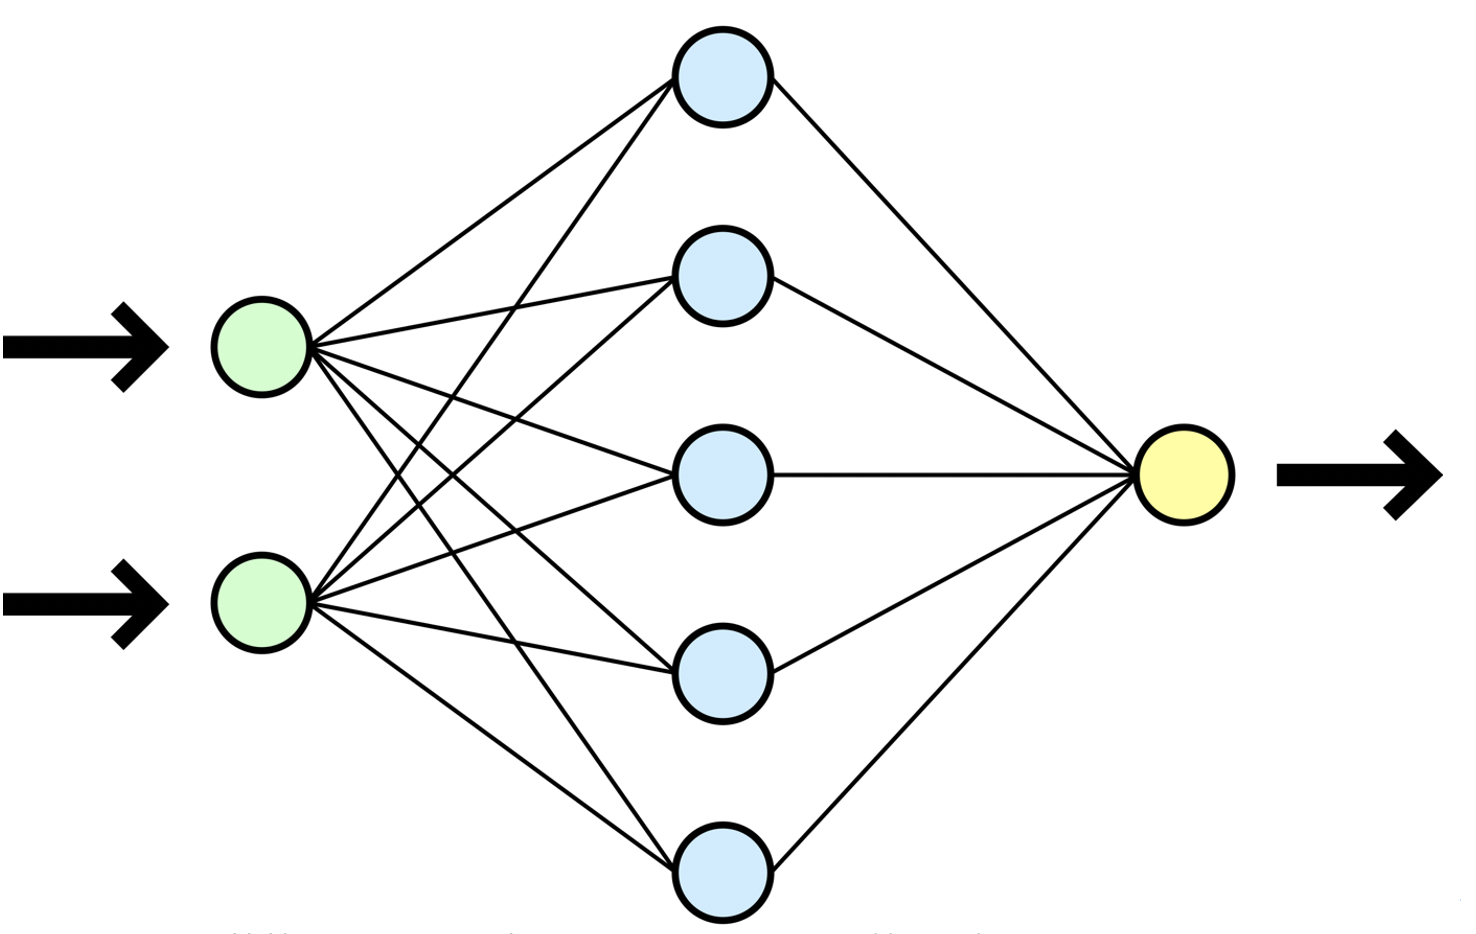
\includegraphics[scale=0.5]{content/pics/Picture_3.png}
\caption{Ein neuronales Netz mit je einem Input-, Hidden- und Output-Layer, aus \cite{Nielsen}}
\label{Abbildung:Nielsen}
\end{figure}

Es gibt neben ANNs und DNNs noch weitere Architekturansätze zur Realisierung von neuronalen Netzen. Einige davon, wie Recurrent Neural Networks (RNNs), sind für bestimmte Aufgaben besser geeignet als andere. RNNs sind insbesondere für die Verarbeitung von natürlicher Sprache von Bedeutung. Es können verschiedene Formen von RNNs unterschieden werden, wobei für den Anwendungsfall der Sprachverarbeitung insbesondere Encoder-Decoder-RNNs hervorzuheben sind, die auch als seq2seq-Modelle bezeichnet werden und besonders gut mit Sequenzen (z. B. Abfolgen von Wörtern) umgehen können. Gemeint ist hier etwa eine Übersetzung, die eine Sequenz als Eingabe benötigt und eine Übersetzung als Sequenz wieder ausgibt. \cite[23-28]{White} Convolutional Neural Networks (CNNs) sind hingegen unter anderem für den Bereich Computer Vision (Bildverarbeitung/ Bilderkennung) von großer Bedeutung. Sie wurden explizit für diese Aufgabe entwickelt \cite[]{LeCun}.

Die verschiedenen neuronalen Netze haben die Gemeinsamkeit, dass sie Neuronen (Knoten) und gewichtete Verbindungen (Kanten) zwischen den Neuronen beinhalten. Neuronen werden aktiviert durch Eingaben und verarbeiten diese mit bestimmten Funktionen weiter, um wiederum eine Ausgabe zu generieren. Das Ermitteln der Gewichtungen dieser Verbindungen wird als Training bezeichnet. Das Training des Netzes besteht aus dem Lösen eines hoch-dimensionalen, nichtlinearen, nicht-konvexen und globalen Optimierungsproblems. Es kann erfolgen unter Zuhilfenahme der Algorithmen Gradient Descent und Backpropagation \cite[1-13]{White}.

Während bei herkömmlichen Machine-Learning-Ansätzen Features (auch: Attribute oder Eigenschaften von Datensätzen), die während der Verarbeitung benötigt werden, manuell von Menschen gebildet werden müssen, werden diese Features bei Deep-Learning-Ansätzen durch das neuronale Netz erzeugt \cite[S. 3-4]{Alom}. Durch diesen Vorteil sind bessere Ergebnisse möglich \cite[S. 11]{Alom}. 

\section{Natural Language Processing}

Es geht nachfolgend um Techniken zur Verarbeitung und Auswertung von Texten und natürlicher Sprache (Engl.: Natural Language Processing, Abk.: NLP).  NLP kann dabei als Teil des umfangreichen Gebiets Text Mining verstanden werden \cite[S. 17]{Perez}. Das Verständnis von natürlicher Sprache (Engl.: Natural Language Understanding, Abk.: NLU) gilt als Voraussetzung für die Schaffung eines vollständigen KI-Systems, wodurch der Bezug von Sprachverständnis bzw. der Sprachverarbeitung zur KI gegeben ist \cite[S. 8]{Yampolskiy}.

\subsection{Vorverarbeitung von Texten}

Eine geeignete Vorverarbeitung (Engl.: Preprocessing) von Texten gilt als Voraussetzung für den Erfolg der späteren Auswertungen \cite[S. 46]{Anandarajan}. Daher werden hier zunächst einige der gängigen Schritte zur Vorverarbeitung von Texten skizziert und grundlegende Methoden erläutert.

Bei der Token-Erstellung (Engl.: Tokenization) wird Text in sogenannte Tokens unterteilt. Im einfachsten Fall bestehen Tokens aus einem Wort – dann handelt es sich um Unigramme (Engl.: unigram). N-Gramme (Engl.: n-grams) stellen eine Alternative zu Unigrammen dar. N-Gramme sind Wort-Sequenzen mit der Länge n \cite[S. 48]{Anandarajan}. Stoppworte dienen zwar einem grammatikalischen Zweck, in Bezug auf den Inhalt von Texten erbringen sie aber nur einen geringen Mehrwert. Aus diesem Grund werden Stoppworte im Rahmen der Vorverarbeitung in der Regel aus Texten entfernt. Dazu kann z. B. ein Wörterbuch verwendet werden, das bekannte Stoppworte wie z. B. [und, er, ein, hat, …] enthält \cite[S. 50-53]{Anandarajan}. Die Reduktion von Begriffen auf die Stammform (Engl.: Stemming) verfolgt das Ziel, verschiedene grammatische Varianten des gleichen Wortes zu vereinheitlichen, um die Gesamtanzahl der unterschiedlichen Wörter innerhalb eines Textkörpers zu reduzieren. Die Erzeugung der Stammformen erfolgt z. B. durch den Porter-Stemmer, der Stammformen auf Basis von Regeln bilden kann. Die Lemmatisierung (Engl.: Lemmatization) führt Begriffe auf eine Art ``Wörterbuchform`` zurück und kann dadurch besser interpretierbare Ergebnisse liefern als das Stemming \cite[S. 30-32]{Manning} Worttypen wie Adjektive, Verben, Substantive, etc. werden erkannt und markiert durch Part-of-Speech-Tags (Abk.: POS-Tags). Zur Realisierung dieser Markierung können Text-Korpora verwendet werden, bei denen manuell Wörter mit den entsprechenden Wortarten markiert wurden \cite[S. 58]{Anandarajan}.

\subsection{Repräsentation von Texten} 

Nach den beschriebenen Schritten zur Vorverarbeitung von Textdokumenten kann die Darstellung von Begriffen im Verhältnis zu Dokumenten über eine Term-Document-Matrix (TDM) erfolgen (vgl. Tabelle \ref{tab:tdm}). Die transponierte Variante dieser Matrix heißt Document-Term-Matrix (DTM) \cite[S. 61ff]{Anandarajan}. Eine TDM könnte so etwa nach der initialen Vorverarbeitung aussehen.

\begin{table}[h]
\centering
\begin{tabular}{|c|c|c|c|c|}
\hline
\textbf{}     & \textbf{Dokument\_1} & \textbf{Dokument\_2} & \textbf{Dokument\_3} & \textbf{...} \\ \hline
\textbf{dog}  & 0                    & 0                    & 2                    & ...          \\ \hline
\textbf{cat}  & 1                    & 1                    & 0                    & ...          \\ \hline
\textbf{bird} & 3                    & 0                    & 1                    & ...          \\ \hline
...           & ...                  & ...                  & ...                  & ...          \\ \hline
\end{tabular}
\caption{Beispiel für eine TDM. Fiktives Beispiel in Anlehnung an \cite[S. 62]{Anandarajan}}
\label{tab:tdm}
\end{table}

In dieser Art der Darstellung wird die Menge der Wörter eines Dokuments als Bag-of-Words bezeichnet \cite[S. 46]{Anandarajan}. Die Ausprägungen in den Zellen der Tabelle \ref{tab:tdm} beschreiben in diesem Beispiel die Häufigkeit des Vorkommens der Begriffe in den jeweiligen Dokumenten. Um zur Term Frequency (Abk.: tf) zu gelangen, ist die Anzahl des Begriffs durch die Gesamtanzahl der Begriffe im jeweiligen Dokument zu dividieren. Für den Begriff cat ergibt sich für Dokument\_1 (erste Spalte) eine tf von \( \frac{1}{4} \), unter Vernachlässigung der Spalten und Zeilen ohne kardinale Ausprägungen (Spalten und Zeilen mit Ausprägung ``...``).

Eine weitere, für die spätere Auswertung relevante Kennzahl heißt Document Frequency (Abk. df). Dabei wird zunächst die Häufigkeit der Begriffe reduziert auf eine binäre Angabe 1 oder 0, die Häufigkeit wird also vernachlässigt und es verbleibt lediglich eine Information darüber, ob ein Wort in den Dokumenten vorkommt oder nicht. Die nun erzeugten Werte werden zeilenweise addiert, um die Kennzahl df zu erhalten. Das Beispiel ``cat`` aus Tabelle \ref{tab:tdm} würde zu einer df von 1+1+0=2 führen. Der Wert df gibt damit an, in wie vielen Dokumenten ein Begriff vorkommt. Um seltenen, und damit aussagekräftigen Begriffen ein höheres Gewicht zu geben als Begriffen, die zwar häufig vorkommen, dafür aber auch weniger Relevanz und Wirkung haben, existiert mit der inversen Dokumenten-Häufigkeit (Engl.: inverse document frequency, Abk.: idf) eine weitere Metrik. Sie wird berechnet als:

\[ idf_i = \log_2( \frac{n}{df_i}) + 1 \]

wobei n die Anzahl der Dokumente ist, und df wie oben beschrieben berechnet wird. Die hier beschriebenen Metriken können kombiniert werden zur tf-idf-Metrik. Dabei wird tf mit idf lediglich multipliziert. Für den Beispielbegriff cat ergibt sich unter Vernachlässigung der Spalten und Zeilen ohne kardinale Ausprägungen ein Wert von \( \frac{1}{4} \times ( \log_2( \frac{3}{2} )+1)=0,39 \) 
für das erste Dokument. Der tf-idf-Wert von Begriffen kann nun als Ausprägung in den Zellen einer TDM an Stelle der schlichten Anzahl der Begriffe verwendet werden \cite[S. 61-73]{Anandarajan}.

Die tf-idf-Metrik ist bei der Betrachtung von mehreren Begriffen zusammengefasst eine Grundlage für die Erkennung von wichtigen Begriffen. Dabei sollten die Dokumente möglichst einen Bezug zueinander haben. Ein Beispiel wäre eine Menge von Dokumenten über Software-Entwicklungsprojekte. In jenen Dokumenten würde der Begriff ``Software`` häufig vorkommen. Die Bedeutung des Begriffs ist allerdings eher gering, da er wahrscheinlich in allen Dokumenten vorhanden sein wird. Beim tf-idf-Maß erhalten seltene Begriffe einen hohen Wert, wodurch solche Begriffe als interessant identifiziert werden können. \cite[S. 107-110]{Manning}. Auf Basis der einfachen TDM oder auch auf Basis der erweiterten Variante unter Verwendung von tf-idf-Werten können im Anschluss Verfahren des maschinellen Lernens verwendet werden, wie im praktischen Teil der Arbeit gezeigt wird.  

\subsection{Regelbasierte Ansätze}

Um ein ML-Modell trainieren zu können, sind Trainingsdaten notwendig (vgl. Kapitel 2.1). Wenn diese nicht in ausreichender Menge vorhanden sind, dann kann ein regelbasierter Ansatz eine Alternative zu Verfahren des maschinellen Lernens sein. Regelbasierte Systeme zählen zu den ältesten Ansätzen im Bereich NLP und haben sich in der Praxis bewährt. Aus technischer Sicht können für die Realisierung eines regelbasierten Ansatzes etwa String-Vergleiche (z. B. mit regulären Ausdrücken zur Entdeckung bestimmter Muster) verwendet werden. Auch mit kontextfreien Grammatiken können Regeln ausgedrückt werden \cite{kaggle}. Ein simpler endlicher Automat kann verwendet werden, um einfache Regeln zu beschreiben \cite[S. 219]{Manning}. Zu den regelbasierten Ansätzen werden hier explizit auch Wenn-Dann-Regeln gezählt \cite[S. 23ff.]{Ertel}. Beispiele für Entitäten, die gut über einen regelbasierten Ansatz erkannt werden können, sind etwa IP-Adressen, URLs, oder Telefonnummern \cite{spacy}.

Über Ontologien oder Taxonomien können ebenfalls Entitäten erkannt werden. Solche Wissensbasen galten früher als grundlegender Baustein von KI-Systemen. Ein solcher Bestand kann zu Beginn eines Projekts erstellt werden und dann im Laufe der Zeit weiterentwickelt werden. Ontologien führen in diesem Kontext zu wiederverwendbaren, erweiterbaren Wissensbeständen. Sie können sowohl von Menschen als auch von Computern verstanden werden und bilden Mengen von explizit definierten Terminologien ab. Die grundlegenden Begriffe, also das Vokabular einer bestimmten Domäne und die Beziehungen der Begriffe untereinander werden in einer Ontologie modelliert \cite[S. 37-55]{ontologies}. Das Vokabular könnte in den erwähnten Wenn-Dann-Regeln verwendet werden. Die Begriffe Ontologie und Topic werden in der Literatur und daher auch hier als Synonyme verwendet. 

Taxonomien können ebenfalls für solche Klassifizierungszwecke verwendet werden. Eine Taxonomie hat einen Namen und besteht aus Beispielen. Es kann flache bzw. einfache Taxonomien geben, aber auch hierarchische, oder gar vernetzte Taxonomien \cite{inmon}

Da im Titel dieser Arbeit die Evaluation von ausgewählten ML-Verfahren festgelegt ist, werden regelbasierte Ansätze im praktischen Teil der Arbeit weniger ausführlich betrachtet als ``echte`` ML-Ansätze. Sie gelten aber in realen Szenarien als mögliche Option für bestimmte Anwendungsfälle und wurden daher hier beschrieben.

\subsection{Vektorbasierte Ansätze}

Die Begriffe Wort-Vektor und Wort-Einbettung (Engl.: Word Embedding) werden hier als Synonyme verwendet, wie in \cite[S. 38]{White}. Als moderner Algorithmus zur Erzeugung von Wort- Einbettungen gilt Word2Vec. Entwickelt wurde das Verfahren von Google-Forschern \cite{mikolov2013}, allerdings sind auch andere Unternehmen an der Weiterentwicklung dieser Ansätze beteiligt. So gibt es etwa mit fastText von Facebook oder mit GloVe der Stanford University ebenfalls Möglichkeiten zur Nutzung von vorbereiteten Word-Vektoren sowie für das Training eigener Wort-Vektoren \cite{facebook} \cite{stanford}. Word2Vec versucht, die Probleme des Bag-of-Word-Ansatzes beziehungsweise der One-Hot-Encodings zu vermeiden. Durch diese Repräsentation – bei der das Vorhandensein eines Wortes in einem Textdokument etwa mit einer 1 angezeigt wird und das Fehlen mit einer 0 – entstehen hoch-dimensionale Tabellen mit vielen Zeilen. Dabei kommt häufig der Wert 0 als Ausprägung vor. Damit einher geht ein gewisser Informationsverlust, da Kontextinformationen (z. B. die Position der Wörter innerhalb der Dokumente) verloren gehen  und weil viele ML-Verfahren mit Daten, die in dieser Art und Weise repräsentiert sind, schlecht umgehen können. Zu viele Spalten können zu einem zu zu komplexen Modell führen, was nicht erwünscht ist \cite[S. 145]{knime}. Als Architektur für das Erzeugen von Wort-Vektoren kommt bei Word2Vec ein voll-verknüpftes neuronales Feed-Forward-Netz zum Einsatz. Eine Eigenschaft des Verfahrens ist, dass bei jedem Wort der Kontext des Worts in gewissem Maße erhalten bleibt. Die Anwendung von Word2Vec führt zu den sogenannten Einbettungen, was letztendlich einer deutlich kompakteren Darstellung der Informationen entspricht, als das etwa bei der Darstellung von Text in Form einer Term-Document-Matrix der Fall ist. Eine Einbettung entspricht einer Darstellung von Begriffen in Vektorform. Die mit Word2Vec erzeugten Wort-Vektoren können als Eingabe für weitere Machine-Learning-Verfahren verwendet werden, wobei diese Repräsentation deutlich bessere Resultate etwa bei Klassifizierungsaufgaben verspricht, als in der unverarbeiteten Form. Um die Vektoren zu erzeugen, wird ein neuronales Netz trainiert, welches das Ziel hat, die Wahrscheinlichkeit von bestimmten Kontextwörtern einzelner Wörter vorherzusagen (im sogenannten Skip-Gram-Ansatz). Die internen Gewichtungen des neuronalen Netzes werden letztendlich als Wort-Vektoren verwendet \cite[S. 148-160]{knime}. 

Neben Wort-Einbettungen kommen an dieser Stelle noch Dokumenten-Einbettungen in Betracht. Der Algorithmus dazu heißt Paragraph Vector. Im Vergleich zu Word2Vec werden für das Erstellen der Einbettungen zusätzlich zu den Wörtern auch jeweils Paragraphen in das Training der Vektoren mit einbezogen. Die Paragraphen liefern also zusätzlichen Kontext. Vergleichbar ist der Paragraph mit einer Angabe darüber, wo im Dokument bzw. auch in welchem Dokument sich ein Begriff in den Trainingsdaten befunden hat \cite{mikolov2014}. Eine Implementierung von Dokument-Einbetttungen findet sich unter dem Namen doc2vec \cite{rehurek}.

In Abbildung \ref{Abbildung:mikolov} dargestellt sind einzelne Wörter, die als Vektoren abgebildet werden. Die Abkürzung W steht aus mathematischer Sicht für eine Matrix, die einzelnen Wort-Vektoren sind als Spalten in dieser Matrix enthalten. Nach Bildung der initialen Vektoren werden diese konkateniert (``aufsummiert``), um den sogenannten Kontext abzubilden. In diesem Beispiel wird ein neuronales Netz verwendet, das die Wahrscheinlichkeit des Wortes ``on`` im Kontext der Begriffe ``the cat sat`` ermittelt. Hier dargestellt ist das Continuous Bag of Word-Modell (CBOW), das genaue Gegenteil von Skip-Gram, das oben bereits erwähnt wurde. Bei der Verwendung des Paragraph-Vector-Ansatzes wird jeder Paragraph als Spalte in einer Matrix D abgebildet. Diese zusätzliche Information ergänzt den beschriebenen Kontext. Was genau als Paragraph definiert wird, kann frei gewählt werden. Es kann sich um längere Abschnitte, ganze Dokumente, oder auch eine Auswahl von Sätzen handeln \cite{mikolov2014}.
 
\begin{figure}[h]
\centering
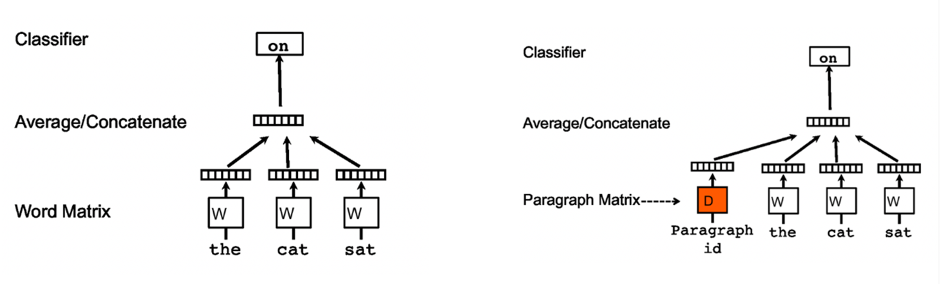
\includegraphics[scale=0.9]{content/pics/Picture_5.png}
\caption{Funktionsweise von Word2Vec (links) und von Paragraph Vector (rechts), aus \cite{mikolov2014}}
\label{Abbildung:mikolov}
\end{figure}

Einbettungen müssen nicht für jede Anwendung neu trainiert werden. Stattdessen können auch vor-trainierte (pre-trained) Einbettungen wiederverwendet werden, wie am Anfang dieses Abschnitts bereits angedeutet wurde. Unten dargestellt (Abbildung \ref{Abbildung:word_vecs}) ist ein Ausschnitt aus dem bereits trainierten GloVe-Modell, der die Vektor-Repräsentation verdeutlichen soll. Es wurde trainiert auf Basis des Korpus Wikipedia 2014 \cite{stanford}. Die Abbildung soll verdeutlichen, dass mit den Vektoren eine mathematische Repräsentation von Begriffen gefunden wurde. Die Wörter können damit für verschiedene Rechenoperationen verwendet werden. Einige davon werden im praktischen Teil dieser Arbeit erprobt. 

\begin{figure}[h]
\centering
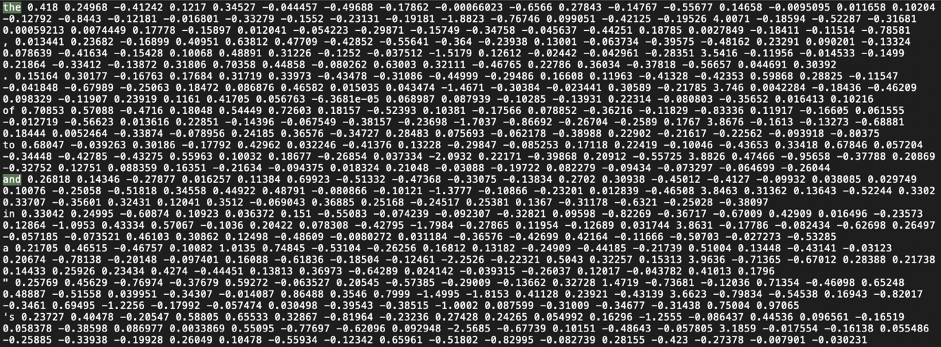
\includegraphics[scale=0.9]{content/pics/Picture_6.png}
\caption{Vektoren der Begriffe ``the`` \& ``and``. Eigene Bildschirmaufnahme.}
\label{Abbildung:word_vecs}
\end{figure}
 
Die größeren NLP-Modelle, etwa von spaCy, beinhalten standardmäßig nutzbare Wortvektoren. Eine eigene Untersuchung ergibt, dass diese Modelle auch gewisse fachspezifische Wörter berücksichtigen, etwa die Begriffe Shipments oder containerization. Allerdings existieren für reale Begriffe wie Projekt- oder Systemnamen aus einem spezifischen Unternehmen keine Wortvektoren. Solche Begriffe nennt man out-of-vocabulary \cite{spacy2}. Das erschwert die Verwendung von Modellen, die ``gebrauchsfertig`` zur Verfügung stehen. 

\subsection{Transformer-Ansätze}
Transformer werden erstmals Ende 2017 eingeführt. Laut den Autoren der Erstveröffentlichung ist der Ansatz in der Lage, bessere Ergebnisse in bestimmten Bereichen zu erzielen als bisherige Ansätze auf Basis von RNNs oder CNNs; zudem ist das Training parallelisierbar und damit schneller als bei früheren Ansätzen \cite{Vaswani}. Transformer-Ansätze können für viele NLP-Teilbereiche verwendet werden, etwa für Named-Entity-Recognition, Übersetzungen, das Generieren von Zusammenfassungen, und weitere Anwendungsfälle. \cite[S. 25-26]{Gupta}. Die Nutzung von vortrainierten Modellen wird als Transfer-Learning bezeichnet. Transformer können dies ermöglichen. Gewisse Gewichtungen innerhalb von neuronalen Netzen können dabei übernommen werden und müssen nicht neu trainiert werden (z. B. grundlegende Sprach-Eigenschaften). Vortrainierte Modelle sind eine Option, wenn nur wenige Daten für das Training zur Verfügung stehen. Die vor-trainierten Modell erfahren eine Fein-Abstimmung (Engl.: Fine-Tuning), wodurch die Modelle an den jeweiligen Anwendungsfall angepasst werden \cite[S. 45-56]{Alom}.
Ein konkreter Transformer-Ansatz ist BERT (Bidirectional Encoder Representations from Transformers). Es gibt eine Pre-Training-Phase und eine Fine-Tuning-Phase, durch die das finale Modell erzeugt wird. Es wurden Ergebnisse in diversen NLP-Referenzproblemen (Beispiel: Beantwortung von Fragen) erreicht, die als state-of-the-art bezeichnet werden können \cite{devlin}. 
GPT (Generative Pre-trained Transformer) und seine Nachfolger GPT-2 und GPT-3 sind weitere Beispiele für Transformer-Modelle, die insbesondere für die Text-Erzeugung eingesetzt werden können \cite{Brown}

\section{Das Application-Portfolio-Management als Teil der IT-Governance}

IT-Governance soll sicherstellen, dass Informationstechnologie (IT) die Strategien und Ziele von Unternehmen unterstützt. Die IT soll so angepasst und weiterentwickelt werden, dass relevante Anforderungen erfüllt werden. Dazu zählen insbesondere regulatorische und gesetzliche Anforderungen \cite[S. 5]{reiss}. Gemeint sind damit etwa Gesetze und Rechtsverordnungen, wie die Datenschutzgrundverordnung (DSGVO), der Sarbanes-Oxley-Act (SOA), oder auch die bankaufsichtlichen Anforderungen an die IT (BAIT) im Bankenumfeld \cite[S. 274-275]{gaulke}. 

Außerdem kann davon ausgegangen werden, dass Manager stets auch weitere, individuelle Interessen aus ihrem Arbeitskontext im Sinn haben, wenn die Notwendigkeit von IT-Governance begründet werden soll. Risiken, die mit dem Betrieb von IT-Systemen einhergehen, sollten dem Management bekannt sein, damit entsprechende Maßnahmen getroffen werden können. Außerdem ist von Interesse, welchen fachlichen Mehrwert einzelne Systeme tatsächlich bringen und welche Geschäftsbereiche durch die Systeme unterstützt werden. Der große Vorteil von IT-Governance ist erhöhte Transparenz. Die Transparenz macht unter anderem Kosten sichtbar und ermöglicht sinnvolle Entscheidungen im Zusammenhang mit der Unternehmens-IT  \cite[S. 5-7]{ncc}. Mit den angesprochenen Risiken können (u. a.) wirtschaftliche Verluste im Falle von Systemausfällen verbunden sein, aber auch der langfristige Verlust der eigenen Wettbewerbsfähigkeit, wenn zu lange mit der Erneuerung von Systemen gewartet wird  \cite[S. 20]{ncc}. IT-Governance ist ein Bestandteil eines übergeordneten Corporate-Governance-Ansatzes, bei dem es um die Steuerung und Überwachung eines gesamten Unternehmens geht \cite[S. 2]{gaulke}. 

\subsection{COBIT als mögliche Grundlage für das APM?}

Das Rahmenwerk (Engl.: Framework) COBIT kann als methodische Grundlage für IT-Governance dienen. Die Abkürzung steht für Control Objectives for Information and Related Technology. Die aktuelle Version (während der Bearbeitungszeit dieser Arbeit) ist COBIT 2019 \cite[S. 9-12]{gaulke}. 

COBIT definiert in seinem Kern-Modell (vgl. Abbildung \ref{Abbildung:isaca}) sogenannte Governance- und Management-Ziele \cite[S. 67]{gaulke}. Ziel APO05 heißt ``Managed Portfolio``. Anhand dieses Beispiels soll verdeutlicht werden, dass der Umgang mit bestimmten Portfolios ein wesentlicher Bestandteil von Governance-Tätigkeiten sein kann. Die Bezeichnung Application-Portfolio wird hier allerdings nicht verwendet, sondern es geht stattdessen um Projekte und Programme. Dabei müssen einzelne Projekte oder Programme priorisiert werden, damit strategische Ziele erreicht werden können \cite[S. 87-92]{isaca1}. 

Statt einem eigenen Management-Ziel zum Umgang mit Applikationen exisitert in COBIT die Empfehlung zu ``Managed Assets`` (``Betriebsmitteln``, vgl. Ziel BAI09) \cite[S. 209-214]{isaca1}, wozu auch der Umgang mit Software-Lizenzen zählt. Unter dem Ziel ``Managed Configuration`` (BAI10) wird empfohlen, Daten zu ``wichtigen Ressourcen`` zu erheben und zu verwalten \cite[S. 73]{gaulke}. Unter Ziel APO03 wird das Managen der Unternehmensarchitektur empfohlen, was die Einrichtung einer Referenzarchitektur beinhaltet, in der u. a. auch Anwendungen und Technologien berücksichtigt werden können \cite[S. 70]{gaulke}. In welchen Variationen diese Empfehlungen in Unternehmen ganz konkret umgesetzt werden, ist diesen stets selbst überlassen \cite[S. 65]{gaulke}.
 
\begin{figure}[h]
\centering
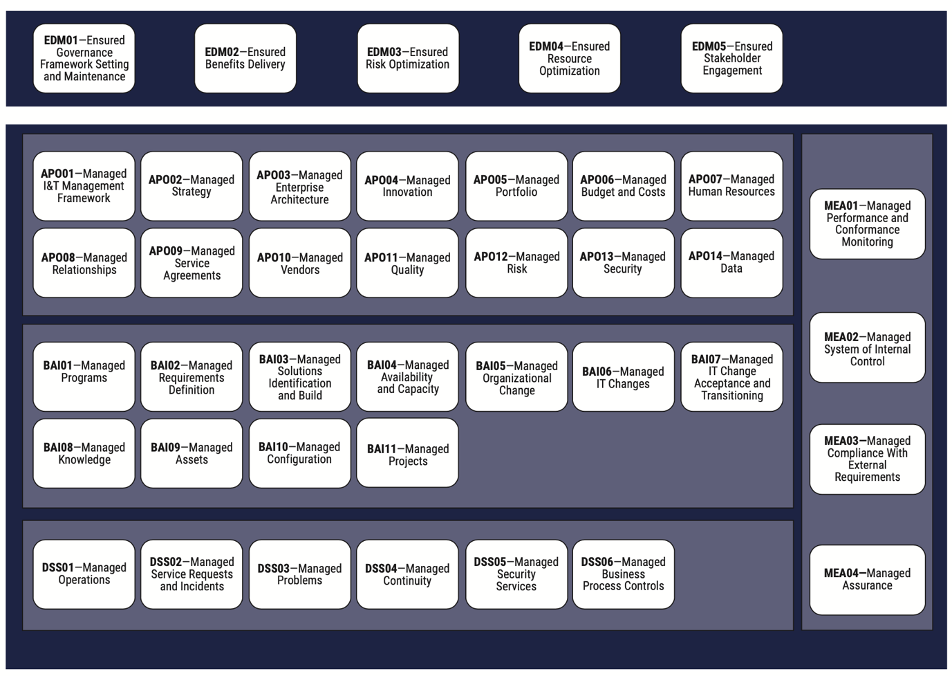
\includegraphics[scale=0.9]{content/pics/Picture_7.png}
\caption{COBIT-Kernmodell, aus \cite[S. 21]{isaca2}}
\label{Abbildung:isaca}
\end{figure}

Neben COBIT gibt es weitere Frameworks, bzw. Modelle zum Umgang mit einzelnen Governance-Themen. In \cite[S. 127-133]{gaulke} werden beispielsweise das CMMI - Capability Maturity Model (Integration) sowie die IT Infrastructure Library (ITIL) erwähnt. 
 
Außerdem gibt es spezielle (Enterprise-)Architektur-Frameworks. Auf einige davon wird in einem späteren Abschnitt kurz eingegangen. 

\subsection{Die Rolle von Textdokumenten für die IT-Governance}
Verschiedene IT-Projekte eines Unternehmens und damit verbunden auch Softwareentwicklungsprojekte stehen grundsätzlich in Konkurrenz zueinander. Mehrere Stakeholder möchten, dass ihr eigenes Projekt mit Priorität behandelt wird und erfolgreich umgesetzt wird. Dazu kommt, dass es Abhängigkeiten zwischen den einzelnen Vorhaben geben kann (Beispiel: Der Abschluss von Projekt A ist eine Voraussetzung für die erfolgreiche Umsetzung von Projekt B). Aus diesem Grund ist es wichtig, dass das IT-Management die Gesamtheit der Projekte im Blick hat, und sich weniger nur auf einzelne Projekte fokussiert \cite[S. 1]{frey}. Ein Portfolio muss also verwaltet und gesteuert werden.

Neben dem voraussichtlichen Return on Investment (ROI) der sich durch die Umsetzung eines Projekts ergibt, müssen weitere Faktoren vor der Umsetzung von Projekten geschätzt werden. Dazu zählt das Risiko, das mit einem Projekt einhergeht \cite[S. 120ff.]{gadatsch}. Zunächst können für diese Schätzung die bereits erstellten Dokumentationen in Betracht gezogen werden. Der Begriff der Dokumentation bezeichnet in der Regel nachträglich erstellte Beschreibungen von Projekten. Unter dem Begriff können allerdings auch die zu einem noch laufenden oder geplanten Projekt gehörenden Dokumente verstanden werden. Dokumentationen erfüllen neben der Aufzeichnung von Ideen in Software-Entwicklungs-Projekten einen weiteren wichtigen Zweck: Sie gelten als wesentliches Werkzeug zur Umsetzung von Governance und zur Sicherstellung von Compliance \cite[S. 2]{reiss}. Diesen Zweck erfüllen sie, wenn Außenstehende die bereits abgeschlossenen oder geplanten Projekte oder Anwendungen bewerten müssen, um letztendlich Entscheidungen zum Umgang mit diesen treffen zu können. Deshalb wird in dieser Arbeit angenommen, dass Dokumentationen in Text-Form von hoher Bedeutung für die Gestaltung der Projekt- und Applikationslandschaft von Unternehmen sind. Die Güte von Dokumentationen ist dabei von entscheidender Bedeutung. Ein Dokumentationsmanagementsystem kann bei der Erstellung von anforderungsgerechten Dokumenten unterstützen. Dabei können verschiedene Vorgaben an die Struktur der Dokumente gemacht werden \cite[S. 29]{reiss}. Dazu zählt beispielsweise eine bestimmte Kapitelstruktur. Diese kann von einer Einteilung der Dokumente zu bestimmten Dokumententypen abhängig gemacht werden \cite[S. 34-39]{reiss}.

\subsection {Das APM und verwandte Begriffe}
Es gibt im Zusammenhang mit der Idee des Application-Portfolio-Management in der Literatur diverse ähnliche Begriffe, die im Kern das beschreiben, was in dieser Arbeit unter APM verstanden wird. Ein solcher Begriff aus einer frühen Veröffentlichung zu APM ist etwa das IT Portfolio Management. Hier wird von stetigen ``Kaufs-, Verkaufs- und Beibehaltungs-Entscheidungen`` gesprochen, um sogenannte IT-Portfolios zu gestalten bzw. um sie stets zu optimieren. APM bildet laut den Autoren gemeinsam mit dem Project Portfolio Management sowie dem IT Asset und Infrastructure Management die Disziplin des IT Portfolio Managements \cite[S. 2-14]{Gliedman}.

Das oben bereits erwähnte Enterprise Architecture Management (EAM) verfolgt einen umfangreicheren, ganzheitlichen Ansatz zur Darstellung, Gestaltung und Weiterentwicklung der gesamten Systemlandschaft von Unternehmen. Es werden sowohl die Prozess- als auch die Systemwelt strukturiert betrachtet. Dabei geht es stets auch um die Schaffung von Transparenz. Durch eine solche Transparenz können etwa unnötig redundante Systeme erkannt bzw. vermieden werden \cite[S. 7-10]{Bitkom}. Mit unnötig redundanten Systemen sind solche Systeme gemeint, welche Geschäftsfunktionen abdecken, die bereits durch andere Systeme oder Anwendungen unterstützt werden. Eine Business Support Matrix kann solche Beziehungen zwischen Anwendungen und Geschäftsfunktionen (auch: Capabilities) visualisieren \cite{jung1}. 
Der Umfang von EAM wird dargestellt in Abbildung \ref{Abbildung:ea}. Die Abbildung soll verdeutlichen, dass der Fokus nicht wie im APM nur auf Applikationen (hier repräsentiert am ehesten durch den Kasten Anwendungsarchitektur) liegt, sondern dass sich EAM mit weiteren Ebenen beschäftigt (etwa mit der Geschäftsarchitektur oder auch mit der Strategie).
 
\begin{figure}[h]
\centering
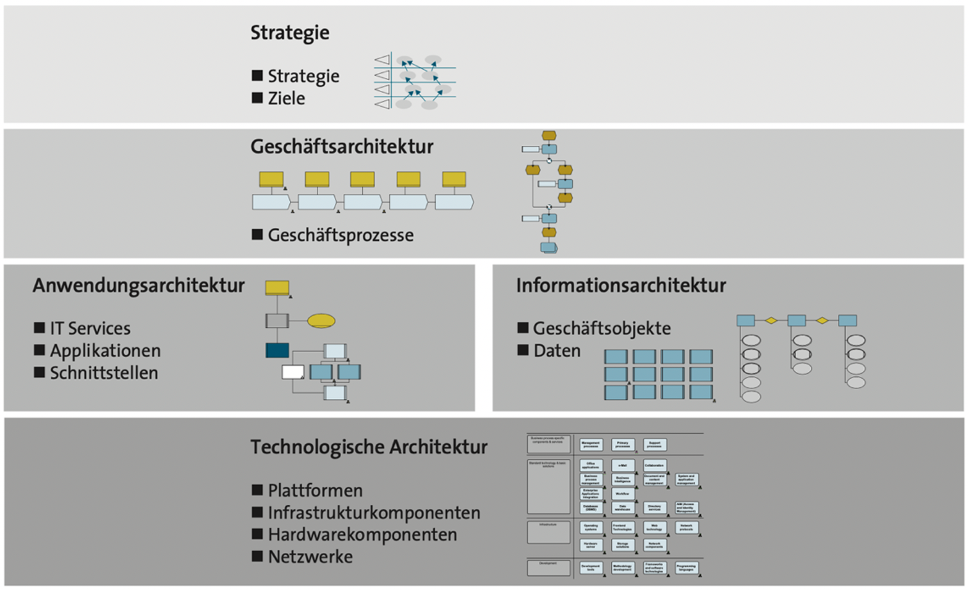
\includegraphics[scale=0.9]{content/pics/Picture_8.png}
\caption{EA-Überblick, aus \cite[S. 13]{Bitkom}}
\label{Abbildung:ea}
\end{figure}

Der enge Bezug von APM und EAM zeigt sich außerdem in Rahmenwerken, wie dem Architekturframework der Open Group (TOGAF). Dort zählt z. B. der Application Portfolio Catalog zu den grundlegenden Artefakten, die bei der Gestaltung einer Architektur nach TOGAF zu berücksichtigen sind. Schnittstellen zwischen Applikationen werden in dem Framework in einem Interface Catalog dokumentiert. Damit sind u. a. Abhängigkeiten visualisierbar und zentrale Anwendungen identifizierbar \cite[Kap. 31]{togaf}. Im Department of Defense Architecture Framework (DoDAF) gibt es verschiedene sogenannte Viewpoints, die wiederum aus mehreren Views bestehen können. Ein Viewpoint in diesem Framework ist die Systems-Viewpoint. Eine konkrete View ist z. B. die ``System Interface Description`` (SV-1). In ihr werden alle Systeme, die von Interesse sind, inklusive Schnittstellen zu anderen Systemen dargestellt. Die View ist vergleichbar mit dem TOGAF Interface Catalog. Es kann in anderen Views auch z. B. um die Unterstützung ``operationaler Aktivitäten`` durch Software-/ oder System-Funktionen gehen (SV-5). Ein Beispiel wäre die Dokumentation darüber, dass der operationale Prozess ``Einchecken von Passagieren``, durch ein System mit der Bezeichnung ``Airline Reservation and Ticketing System`` abgewickelt wird \cite[S. 311-344]{Rao}.

Darüber hinaus zeigt eine Befragung von Enterprise-Architekten, dass diese sich in ihrer täglichen Arbeit mit Fragen zum Umgang mit Anwendungslandschaften beschäftigen \cite{jung2}. Dazu zählen zum Beispiel Fragen wie 

\begin{itemize}
  \item Welche Anwendungen sind in Verwendung? 
  \item Welchen Zweck erfüllen einzelne Anwendungen?
  \item Welche Anwendungen sollen eingeführt oder abgeschaltet werden?
  \item Welche Redundanzen in der Anwendungslandschaft gibt es?
  \item Welche Abhängigkeiten oder Schnittstellen gibt es zwischen Anwendungen?
  \item In welchen Anwendungen werden kritische oder schützenswerte Daten gehalten?
\end{itemize}

Als Kernelement von IT-Strategien wird der IT-Bebauungsplan in einer Veröffentlichung zum Thema IT-Controlling bezeichnet. Er gibt Aufschluss über die Informationssysteme, die derzeit in einem Unternehmen im Einsatz sind. Dazu zählen (u. a.) Informationen zu Release-Ständen, zu Schnittstellen der Systeme untereinander sowie zu Geschäftsprozessen, die die von den Systemen unterstützt werden. \cite[S. 36]{gadatsch} Die Autoren dieses Beitrags nennen das IT-Portfoliomanagement als Werkzeug für IT-Controller (die dem Chief Information Officer gleichgestellt oder dieser Position direkt unterstellt sein können). Zu deren Aufgaben können die Auswahl und Steuerung von neuen Projekten oder von Wartungsprojekten gehören. \cite[S. 41-45]{gadatsch}

\subsection {Handlungsfelder des APM}
Ein grundlegendes Ziel von APM ist die Reduzierung der Komplexität von Anwendungslandschaften. Die fachlichen Anforderungen sollen bestmöglich unterstützt werden durch Anwendungen. Die Gesamtheit der Anwendungen soll jedoch eine möglichst geringe Komplexität aufweisen. Anwendungen werden dabei aus technischer (etwa Aktualität der Software), fachlicher (z. B. Eignung der Software zur Unterstützung der geschäftlichen Anforderungen) und betriebswirtschaftlicher Sicht (Betriebs- oder Lizenzkosten) untersucht. Es handelt sich um einen kontinuierlichen, andauernden Vorgang \cite{schoder}. Nachfolgend aufgelistet sind Beispiele für Fragestellungen, mit denen sich das APM befasst. Sie werden im Folgenden als Handlungsfelder des Application-Portfolio-Management zusammengefasst. Die Fragen wurden abgeleitet aus \cite{apm}. Hervorgehoben sind vier Fragen, auf die im weiteren Verlauf der Arbeit noch stärker eingegangen werden soll. Es gibt auch jeweils einen Verweis auf das jeweilige Kapitel, in denen entsprechende Verfahren zum Umgang mit den Fragen diskutiert werden.

\begin{itemize}
\item Werden bei der Implementierung von neuer Software Legacy-Systeme als Grundlage verwendet?
\item Werden die Anforderungen aus dem operativen Geschäft durch neue Anwendungen abgedeckt?
\item Sind Anwendungen aus technischer und fachlicher Sicht ``fit`` für die Zukunft?
\item Werden durch Anwendungen bestimmte rechtliche Anforderungen umgesetzt?
\item {\bf Was ist für einzelne Anwendungen ``in-scope`` und was ist ``out-of-scope``? (vgl. Abschnitt 4.3)}
\item Gibt es in den Dokumentationen der geplanten Softwareprojekte einen Projektplan oder ein Gantt-Diagramm?
\item {\bf Wurde schon einmal versucht, ein bestimmtes Vorhaben umzusetzen und wie war das Resultat? (vgl. Abschnitt 4.1)}
\item Was sind die fachlichen Anforderungen, die durch ein bestimmtes Projektvorhaben abgedeckt werden sollen?
\item Wie verhalten sich die Kosten, die durch das Ersetzen einer Software anfallen im Vergleich zu den Kosten, die bei einer Modernisierung/ Weiterentwicklung entstehen?
\item Ist es möglich, einzelne Anwendung zu verbessern/ weiterzuentwickeln?
\item Was spricht für eine Wartung einer bestehenden Software, was für eine Neuentwicklung?
\item Welche Anwendungen sind Kandidaten für eine Restrukturierung/ Optimierung
\item {\bf Welche Abhängigkeiten von einzelnen Anwendungen gibt es zu anderen Anwendungen im Application Portfolio? (vgl. Abschnitt 4.4)}
\item Werden bei Neueinführung von Software Abhängigkeiten geschaffen?
\item Welcher Aufwand für die Einführung einer Anwendung ist realistisch?
\item Welche Auswirkungen hat eine Nicht-Verfügbarkeit von einzelnen Anwendungen?
\item In welcher Phase im Lebenszyklus befinden sich bestimmte Anwendungen?
\item Sind Performance-Verbesserungen durch die Einführung von neuer Software identifizierbar?
\item Werden bestehende Prozesse angemessen durch neue/ bestehende Anwendungen unterstützt?
\item Mit welchen Risiken wird die Organisation durch den Betrieb der Anwendungen konfrontiert und wie können die Risiken minimiert werden?
\item Was sind Dinge, die problematisch sein könnten bei Veränderungen am Application Portfolio?
\item Ist ein Produkt auf Basis der eigenen Bedürfnisse neu zu entwickeln oder kann ein Standardprodukt (z. B. für die Zeiterfassung) gewählt werden?
\item In welchen Fällen muss über den Abbruch eines laufenden Projekts nachgedacht werden?
\item Geht es bei Projekten eher um das ``Bekämpfen von Bränden`` (Engl.: ``Firefighting``) oder um echte Verbesserungen der Geschäftsprozesse?
\item {\bf Wie gut ist die Dokumentation einer Anwendung? (vgl. Abschnitt 4.2)}
\item Passen Implementierungsplanungen und strategische Planungen des Unternehmens zusammen?
\item Wie stark werden Standards (z. B. Standard-Entwicklungsmethoden) eingehalten?
\item Wie ist die Aktualität der Anwendungen im Portfolio – welche Anwendungen sind veraltet?
\item Wie lange werden Anwendungen vom Hersteller (Vendor) noch unterstützt (z. B. durch Wartung, Fehlerbehebung, etc.)?
\item Wie ist die Kritikalität von Anwendungen (mission-critical, critical, high, medium, low)?
\item Wer sind die Verantwortlichen (Engl.: ``Owner``) der Anwendungen?
\item Ist die Funktionalität einer Anwendung einzigartig und nicht redundant?
\item Was sind ``Lessons Learned``, die sich ergeben haben durch Betrieb von Software?
\item Wie einfach ist eine Anwendung nutzbar?
\item Welche sind die am häufigsten/ seltensten genutzten Anwendungen im Portfolio?
\item Wie viele Nutzer hat eine Anwendung?
\item Ist die Anwendungslandschaft mit jener von Wettbewerbern vergleichbar?

\end{itemize}

Ein Großteil dieser Fragestellung setzt zur Beantwortung Expertenwissen voraus. Als Beispiel wird die Bezeichnung der ``strategischen Planung`` herausgegriffen. Ein solcher Begriff wäre in der Realität zunächst durch Experten zu definieren. 

\subsection{Unterstützung von APM durch Tools}
Im vorangegangen Abschnitt wurden einzelne Fragen genannt, bei deren Beantwortung Experten durch Technologie unterstützt werden können. Zum einen gibt es dazu die bereits erwähnten Frameworks wie COBIT, TOGAF und weitere – zum anderen gibt es auch spezialisierte Software-Produkte, die an dieser Stelle unterstützen können, wie:

\begin{itemize}
\item ServiceNow Application Portfolio Management. Die unterstützten Anwendungsfälle umfassen u. a. das Darstellen der gesamten Applikationslandschaft, die Verknüpfung von Anwendungen mit Projekten, sowie das Zuordnen von Anwendungen zu Lebenszyklus-Phasen \cite{servicenow}.
\item LeanIX Enterprise Architecture Suite. Die Unterstützung des APM ist einer der grundlegenden Anwendungsfälle des Produkts. Mit dem Werkzeug können (u. a.) Anwendungen mit Business Capabilites verknüpft, Lebenszyklus-Phasen erfasst, und Anwendungslandschaften visualisiert werden \cite{leanix}.
\item Alfabet (Software AG). Sowohl Anwendungsfälle im Bereich EAM als auch im sogenannten Integrated Portfolio Management (ITPM) werden durch die Software abgedeckt. Dabei sind bestimmte Features auch explizit für das APM von Relevanz, wie das Zusammenstellen eines Anwendungs-Inventars, das Zuordnen von Anwendungen zu Lebenszyklus-Phasen, sowie das Hinzufügen von Attributen zu Anwendungen, wie beispielsweise Kosten, Risiken, Nutzungsgrad, und Performance \cite{softwareag}.
\end{itemize} 

All diese Tools sind laut den Herstellern geeignet, um das APM grundlegend zu unterstützen, wobei Inhalte manuell erfasst werden müssen. Die in Word-Dokumenten verborgenen Informationen werten sie jedoch nicht aus. Sie wenden darüber hinaus keine oder kaum Möglichkeiten aus dem Bereich des maschinellen Lernens auf die eigentlichen Inhalte an. Sie nutzen damit das bestehende Potenzial dieser Ansätze noch nicht. Hier sollen die Verfahren ansetzen, die in den nachfolgenden Abschnitten untersucht werden.

